\documentclass[../../../../main.tex]{subfiles}

\begin{document}

\section*{第1問}

{\bf [解]}
点$X$に対し$\overrightarrow{AX}=\vec{x}$とおく．$\vec b=\overrightarrow{AB}$，$\vec d=\overrightarrow{AD}$は互いに一次独立である．

\begin{align*}
\vec e=\frac12\vec b，\quad \vec f=\vec b+\frac23\vec d，\quad \vec g=\frac14\vec b+\vec d
\end{align*}

から，$s,t\in\mathbb{R}$として
\begin{align*}
\vec p&=s\vec e+(1-s)\vec c=\frac12s\vec b+(1-s)(\vec b+\vec d)=\left(1-\frac12s\right)\vec b+(1-s)\vec d，\\
\vec p&=t\vec f+(1-t)\vec g=t\left(\vec b+\frac23\vec d\right)+(1-t)\left(\frac14\vec b+\vec d\right)=\left(\frac14+\frac34t\right)\vec b+\left(1-\frac13t\right)\vec d
\end{align*}

とおける（$\vec c=\overrightarrow{AC}=\vec b+\vec d$）．係数比較して
\begin{align*}
1-\frac12s=\frac14+\frac34t，\qquad 1-s=1-\frac13t
\end{align*}
\begin{align*}
\therefore\ t=\frac{9}{11}，\quad s=\frac{3}{11}
\end{align*}

だから
\begin{align*}
\vec p=\frac{19}{22}\vec b+\frac{8}{11}\vec d
\end{align*}

とおける．$k,\ell\in\mathbb{R}$として
\begin{align*}
\vec q=\vec b+k\vec d=\ell\left(\frac{19}{22}\vec b+\frac{8}{11}\vec d\right)
\end{align*}

とおける．係数比較して$\ell=\dfrac{22}{19}$だから，$\overline{AP}:\overline{PQ}=19:3$．

\begin{figure}[htb]
\centering
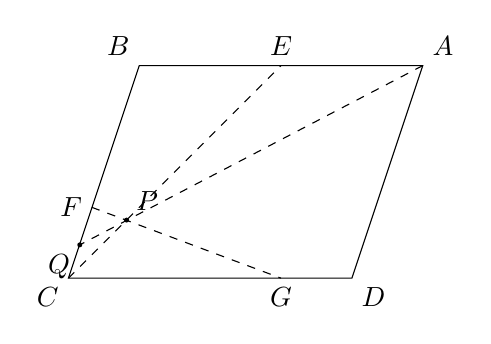
\begin{tikzpicture}[scale=0.9, >=stealth]
  \coordinate (A) at (4,3);
  \coordinate (B) at (0,3);
  \coordinate (C) at (-1,0);
  \coordinate (D) at (3,0);
  \coordinate (E) at (2,3);
  \coordinate (F) at (-0.67,1);
  \coordinate (G) at (2,0);
  \coordinate (P) at (-0.18,0.82);
  \coordinate (Q) at (-0.84,0.47);
  \draw (A) -- (B) -- (C) -- (D) -- cycle;
  \draw[dashed] (C) -- (E);
  \draw[dashed] (F) -- (G);
  \draw[dashed] (A) -- (Q);
  \node[above right] at (A) {$A$};
  \node[above left] at (B) {$B$};
  \node[below left] at (C) {$C$};
  \node[below right] at (D) {$D$};
  \node[above] at (E) {$E$};
  \node[left] at (F) {$F$};
  \node[below] at (G) {$G$};
  \node[above right] at (P) {$P$};
  \node[below left] at (Q) {$Q$};
  \fill (P) circle (1pt);
  \fill (Q) circle (1pt);
\end{tikzpicture}
\caption{平行四辺形$ABCD$と点$E$，$F$，$G$，$P$，$Q$の位置関係}
\end{figure}

\newpage

\section*{第2問}

{\bf [解]}
$N\in\mathbb{N}_{\ge2}$とする．$A_M=\displaystyle\sum_{n=1}^Ma_n$とする．$N=2$の時，$a_1=1$，$a_k=0\ (k\ge2)$から，
\begin{align*}
\max A_M=1\le2^3-2-5=1
\end{align*}
となり成立する．以下$N\ge3$とする．帰納的に，
\begin{align*}
a_1=2^N-3，\quad a_2=2^{N-1}-2，\quad a_k=2^{N+1-k}-1\ (k=3,\ldots,N)，\quad a_k=0\ (N+1\le k)
\end{align*}
となるから，$M=N$の時に題意が成立すれば良い（$a_n\ge0$から，$A_M\le A_N$）．
\begin{align*}
A_N&=(2^N-3)+(2^{N-1}-2)+\sum_{k=3}^N(2^{N+1-k}-1)\\
&=3\cdot2^{N-1}-5+\sum_{k=1}^{N-2}2^k-(N-2)\\
&=3\cdot2^{N-1}-N-3+2\cdot\frac{2^{N-2}-1}{2-1}\\
&=2^{N+1}-N-5
\end{align*}
だから，成立．

以上から題意は示された．$\blacksquare$

\newpage

\section*{第3問}

{\bf [解]}
$n$の時の$a,b$を$a_n,b_n$とする．$x^n=P(x)(x^2-2x-1)+a_nx+b_n$と書ける．両辺に$x$をかけて，
\begin{align*}
x^{n+1}=\left[xP(x)+a_n\right](x^2-2x-1)+(2a_n+b_n)x+a_n\quad\cdots①
\end{align*}
となる．

以下，「$a_n,b_n\in\mathbb{Z}$かつ$a_n\perp b_n$」を◇とし，帰納的に示す．$n=1$の時，$(a_1,b_1)=(1,0)$となり◇成立．以下$n=k$での成立を仮定する．①から
\begin{align*}
a_{k+1}=2a_k+b_k\in\mathbb{Z}，\qquad b_{k+1}=a_k\in\mathbb{Z}\quad\cdots②
\end{align*}
だから，$a_{k+1}$，$b_{k+1}$が共通の素因数$d$を持つとすると，$a_k$，$b_k$も$d$で割り切れ仮定に反する．よって$a_{k+1}\perp b_{k+1}\quad\cdots③$

②③から$n=k+1$でも◇は成立する．以上から示された．$\blacksquare$

\newpage

\section*{第4問}

{\bf [解]}
$f(x)=C+\dfrac{\sqrt3}4x^2$（$C=\cos x$，$S=\sin x$）とおく．$f'(x)=-S+\dfrac{\sqrt3}2x$であり，
\begin{align*}
f''(x)=-C+\frac{\sqrt3}2
\end{align*}
から下表を得る（$f$は偶関数だから，以下$0\le x\le\pi/2$で調べれば良い）．

\begin{center}
\begin{tabular}{c|ccccccc}
$x$ & $0$ & & $\pi/6$ & & $\alpha$ & & $\pi/2$ \\
\hline
$f''$ & & $-$ & $0$ & $+$ & & $+$ & \\
\hline
$f'$ & $0$ & $\searrow$ & $-$ & $\searrow$ & $0$ & $\nearrow$ & $-1+\dfrac{\sqrt3}4\pi$ \\
\hline
$f$ & & $\searrow$ & & $\searrow$ & & $\nearrow$ & \\
\end{tabular}
\end{center}

（$\dfrac{\sqrt3}4\pi-1>\dfrac{1.7}4\cdot3.1-1=\dfrac{1.27}4>0$から，$\dfrac\pi6<\alpha<\dfrac\pi2$かつ$f'(\alpha)=0$を満たす$\alpha$がただ一つ存在する．）

よって，最大値の候補は，$f(0)=1$，$f(\pi/2)=\dfrac{\sqrt3\pi^2}{16}$であり，
\begin{align*}
f\left(\frac\pi2\right)>\frac{1.7\cdot(3.1)^2}{16}=\frac{16.337}{16}>1=f(0)
\end{align*}
から，もとめるのは
\begin{align*}
f\left(\frac\pi2\right)=\frac{\sqrt3\pi^2}{16}．
\end{align*}

\newpage

\section*{第5問}

{\bf [解]}
$C_1:y=\sqrt3\log(x+1)$，$C_2:y=\sqrt3\log(1-x)$である．

円$C$の半径を$r\ (>0)$とすると，$\triangle ABP$が正三角形であるから，$A$，$B$の$x$座標は順に$\dfrac12r$，$-\dfrac12r$である．さらに$P(0,a)$とおくと，$A$での$C_1$の接線$\ell_1$は
\begin{align*}
\ell_1:y=\frac{\sqrt3}{1+\frac12r}\left(x-\frac12r\right)+\sqrt3\log\left(1+\frac12r\right)
\end{align*}
であり，半径$PA\perp\ell_1$かつ$PA$と$y$軸のなす角が$30^\circ$であることから，$\ell_1$の傾きが$\tan30^\circ=\dfrac{\sqrt3}3$だから，
\begin{align*}
\frac{\sqrt3}{1+\frac12r}=\frac{\sqrt3}{3}\quad\therefore\ r=4\quad\cdots①
\end{align*}

この時，$a$を$2$通りで表して
\begin{align*}
a=\sqrt3\log\left(1+\frac12r\right)+\frac{\sqrt3}2r=\sqrt3\log3+2\sqrt3\quad\cdots②
\end{align*}
である．

\begin{figure}[htb]
\centering
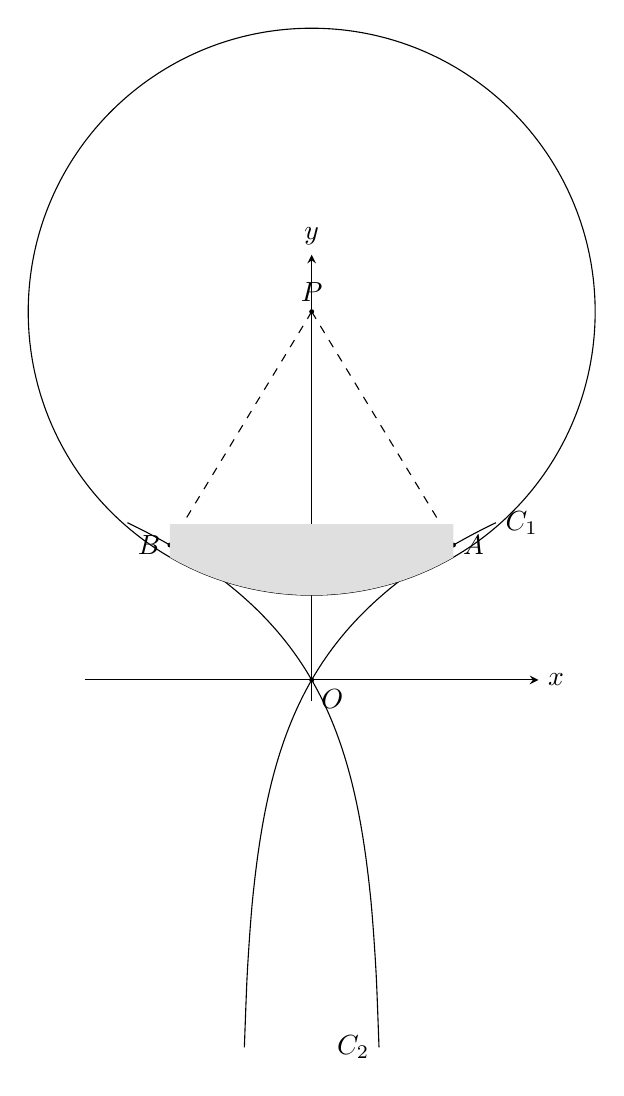
\begin{tikzpicture}[scale=0.9, >=stealth]
  \draw[->] (-3.2,0) -- (3.2,0) node[right] {$x$};
  \draw[->] (0,-0.3) -- (0,6) node[above] {$y$};
  \draw[domain=-0.95:2.6, samples=100, smooth] plot (\x, {sqrt(3)*ln(\x+1)}) node[right] {$C_1$};
  \draw[domain=-2.6:0.95, samples=100, smooth] plot (\x, {sqrt(3)*ln(1-\x)}) node[left] {$C_2$};
  \draw (0,5.196) circle (4);
  \fill (0,5.196) circle (1pt) node[above] {$P$};
  \fill (2,1.903) circle (1pt) node[right] {$A$};
  \fill (-2,1.903) circle (1pt) node[left] {$B$};
  \fill (0,0) circle (1pt) node[below right] {$O$};
  \draw[dashed] (0,5.196) -- (2,1.903);
  \draw[dashed] (0,5.196) -- (-2,1.903);
  \begin{scope}
    \clip (-2,0) rectangle (2,2.2);
    \clip (0,5.196) circle (4);
    \fill[gray!25] (-2.2,-0.2) rectangle (2.2,2.2);
  \end{scope}
\end{tikzpicture}
\caption{円$C$と曲線$C_1$，$C_2$で囲まれた部分（斜線部）}
\end{figure}

求める面積を$S$とする．対称性から
\begin{align*}
\frac12S=(\text{台形}OAP)-(\text{$C_1$と$x$軸，$x=2$で囲まれた部分})-(\text{中心$P$，半径$r$，中心角$\pi/6$の扇形})\quad\cdots③
\end{align*}
であり，
\begin{align*}
\text{台形}OAP&=\frac12\{\sqrt3\log3+a\}\cdot2=\sqrt3\log3+a，\\
\int_0^2\sqrt3\log(x+1)\,dx&=\sqrt3\Bigl[(x+1)\log(x+1)-(x+1)\Bigr]_0^2=\sqrt3(3\log3-2)，\\
\text{扇形}&=\frac12\cdot\frac\pi6\cdot r^2=\frac43\pi
\end{align*}

を②とあわせて③から
\begin{align*}
\frac12S&=2\sqrt3\log3+2\sqrt3-\left(3\sqrt3\log3-2\sqrt3+\frac43\pi\right)\\
&=4\sqrt3-\sqrt3\log3-\frac43\pi
\end{align*}
\begin{align*}
\therefore\ S=2\left(4\sqrt3-\sqrt3\log3-\frac43\pi\right)．
\end{align*}

\newpage

\section*{第6問}

{\bf [解]}
$x$にある石に対し試行を行い，後の座標を$f(x)$とすると
\begin{align*}
f(x)=\begin{cases}-x&(\text{確率}\frac12)\\2-x&(\text{確率}\frac12)\end{cases}
\end{align*}
である．

\textbf{(1)} 2回試行を繰り返すと，以下のようになる．
\begin{itemize}
\item $x\to-x\to x$（確率$\frac12\cdot\frac12=\frac14$）
\item $x\to-x\to2+x$（確率$\frac14$）
\item $x\to2-x\to x-2$（確率$\frac14$）
\item $x\to2-x\to x$（確率$\frac14$）
\end{itemize}

よって，もとめる石置率$P=2\cdot\dfrac14=\dfrac12$．

\textbf{(2)} $2k$回目の試行の後（$k\in\mathbb{N}$）の石の位置を$a_k$とすると，(1)から，
\begin{align*}
a_{k+1}=\begin{cases}a_k&(\text{確率}\frac12)\\a_k+2&(\text{確率}\frac14)\\a_k-2&(\text{確率}\frac14)\end{cases}
\end{align*}
となる．$a_{k+1}=a_k-2$となる試行が1回でも行われた場合，$\max a_n=2(n-1)-2=2n-4$となるから，$a_n=2n-2$は不適である．同様に考えて，$a_n=2n-2$となるのは，$a_{k+1}=a_k$が$1$回，$a_{k+1}=a_k+2$が$n-1$回行われた時であり，もとめる確率は
\begin{align*}
P={}_n\mathrm{C}_1\left(\frac12\right)\left(\frac14\right)^{n-1}=n\left(\frac12\right)^{2n-1}．
\end{align*}

\newpage

\end{document}
